\documentclass[convert]{standalone}
\usepackage{tikz}

\usetikzlibrary{trees,calc}
\usetikzlibrary{intersections}
\usetikzlibrary{positioning}

\tikzset {
    emph/.style = {edge from parent/.style={very thick, draw}},
    norm/.style = {edge from parent/.style={black, thin, draw}}
    %square/.style={regular polygon,regular polygon sides=4}
}

\begin{document}
   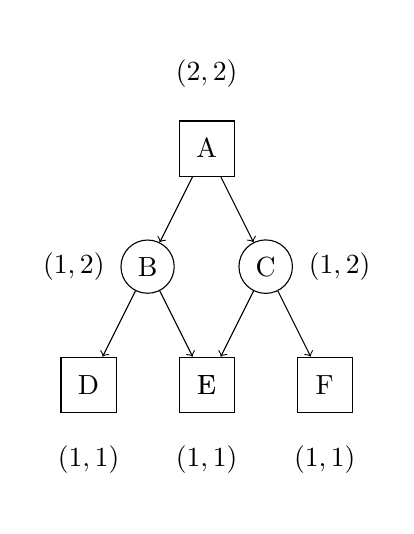
\begin{tikzpicture}[every node/.style={shape=circle, draw=black}, -=->, ->=stealth] 
	\begin{scope}
	\node (a) [label={above:$(2,2)$}, shape=rectangle, minimum height=0.7cm, minimum width=0.7cm] {A} 
	child { node (b) [label={left:$(1,2)$}] {B} 
        child { node (d) [label={below:$(1,1)$}, shape=rectangle, minimum height=0.7cm, minimum width=0.7cm] {D} 
          %  edge from parent node[draw=white, left] {2}
        } 
        child { node (e) [label={below:$(1,1)$}, shape=rectangle, minimum height=0.7cm, minimum width=0.7cm] {E} 
            %edge from parent node[draw=white, left] {1}
        }     
        %edge from parent node[draw=white, left] {1}
	}
	child { node (c) [label={right:$(1,2)$}] {C} 
        child { node (e2) [shape=rectangle, minimum height=0.7cm, minimum width=0.7cm]  {E} 
            %child { node (g) {G} %edge from parent node[draw=white, right] {1} 
            %}
            %edge from parent node[draw=white, left] {1}
        }
        child { node (f) [label={below:$(1,1)$}, shape=rectangle, minimum height=0.7cm, minimum width=0.7cm] {F}  %edge from parent node[draw=white, above right] {3} 
        }
        %edge from parent node[draw=white, right] {1}
    }
	;
    %\draw[thick,-] ($(a)!0.3!(b)$) to[bend right=30] ($(a)!0.3!(c)$);
    %\node [draw=white, above = 0.1cm of k ] {1};
    %\node [below of = g, draw=white] {$G$};
	\end{scope}
	\end{tikzpicture}
	 
\end{document}
